\subsection{Jet Algorithm with Tracks}
\label{sec:TrkJets}

A rapid firmware implemented track clustering algorithm allows to combine an integrated collection of tracks and output a collection of track-based jets. The track-based jets can then be used for globral trigger quantities like $H_{T}$ and $H_{T}^{miss}$. As described in Section~\ref{sec:TkMET}, the same set of track purity requirements are applied to the input selection of tracks to keep the L1 trigger objects resilient to pileup. In this section, we describe the simple track clustering alogirthm that is implemented in firmware. Though the algorithm does not make use of an input L1 primary vertex, it can be used as input to the algorithm to make the algorithm more robust against conaminating L1 tracks from pileup. 

The clustering of tracks in the $\eta$-$\phi$ plane is done using a nearest-neighbor approach in two 1-dimensional steps. The first phase of the algorithm parses tracks into 27 $\phi$ regions and 24 $\eta$ regions, which divides the region of tracking acceptance into cells of that are $\approx 0.2\times 0.2$. The $trk_{z0} $ is also used to assign the track to a z-cell along the beam spot. The clustering in $\eta$-$\phi$ is done in z-regions that span the beamspot. In between every two z-cells is a third cell to cover the overlapping region and eliminate edge cases where the primary vertex is close to the edge of a given bin. This gives a maximal jet size that is approximately a 3x3 square of cells with a half-side equal to $\Delta R=0.3$. The width of the z-cell used for this study is 1cm. 

 Only tracks passing the purity requirements in Table~\ref{tab:trkpurity} are clustered. In the first layer of track clustering in $\phi$, the sum of track $p_{T}$, $\sum p_{T}^{trk}$, in each cell is compared to its two neighbors in $\phi$ and the $p_{T}$ is summed into the local maximum cell. The result of this step is to create a list of 1-dimensional track $\sum p_{T}^{trk}$ clusters based on the local maxima in the $\phi$ dimension, so that the minimum distance between any two $\phi$-clusters is one cell. The next step is to take the $\phi$-clusters and check if cells neighbor each other in $\eta$, and if they do they are merged into the $
\phi$-cluster with larger $\sum p_{T}^{trk}$. The track-based jets are then the list of cells from the local maximum in the $\eta$-$\phi$ plane for a given z-cell. Jets from the primary interaction are found by summing the track-based jet $p_{T}$, $H_{T}^{trk}$, in each z-cell and taking the jets from the z-bin with the largest $H_{T}^{trk}$.  In addition, to the $\sum p_{T}^{trk}$, the track multiplicity is also summed in the same procedure to provide an additional handle for the output collection of track-based jets. This approach gives a list of track-based jet positions in $\eta$,$\phi$, $z_{0}$, $p_{T}$, and $N_{tracks}$.

Figure~\ref{fig:TkJetEfficiency} shows the reconstruction effficiency for this firmware implementable track clustering compared to a full anti-$k_{T}$ clustering with FASTJET. The same set of input L1 reconstructed tracks is used that pass the track purity requirements. The efficiencies are similar across the range of tracking acceptance and the generator level $p_{T}$ range, so the approach of 1D nearest neighbor clustering in two steps gives similar efficieny to full 2D jet reconstruction in an algorithm similar to offline jet reconstruction. 


 

\begin{figure}[htbp!]
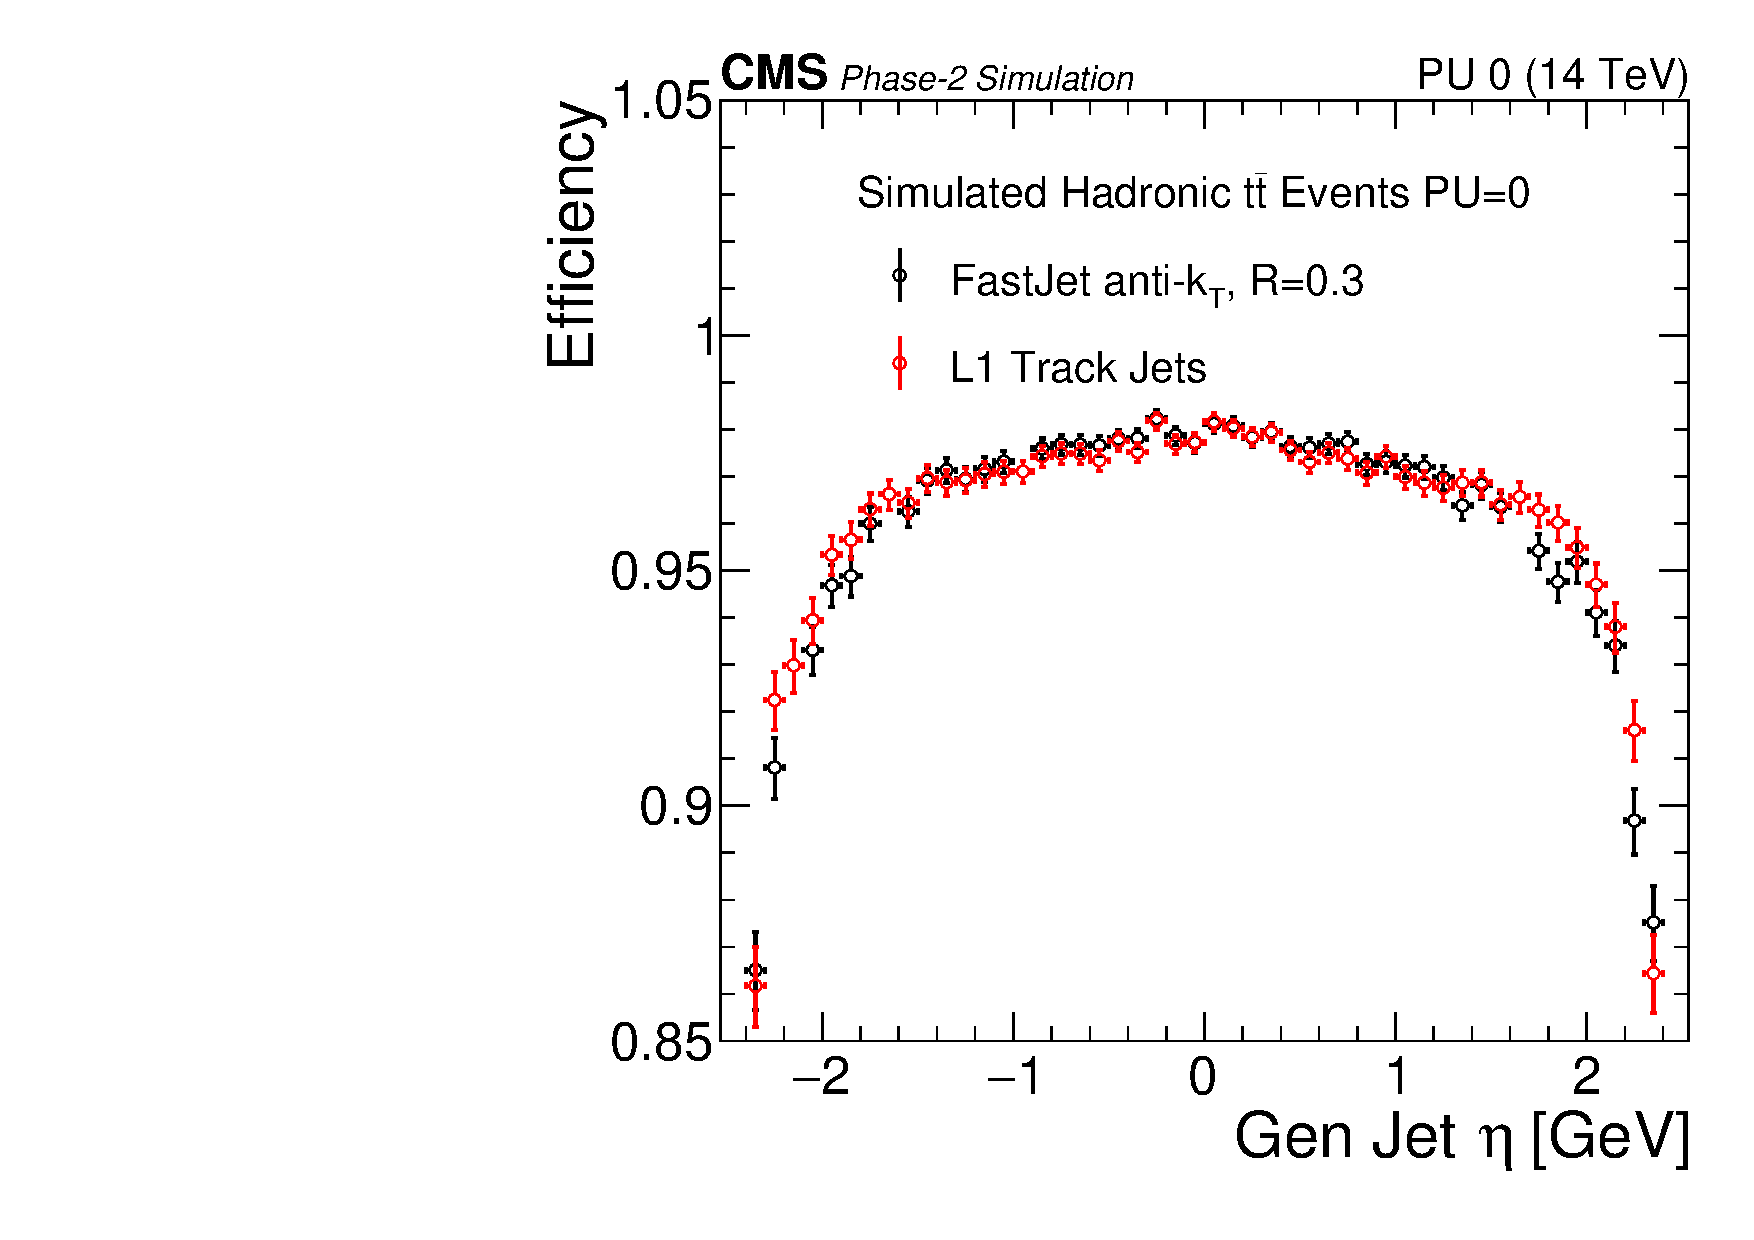
\includegraphics[width=0.45\textwidth ]{NoPUTTBarEff.pdf}
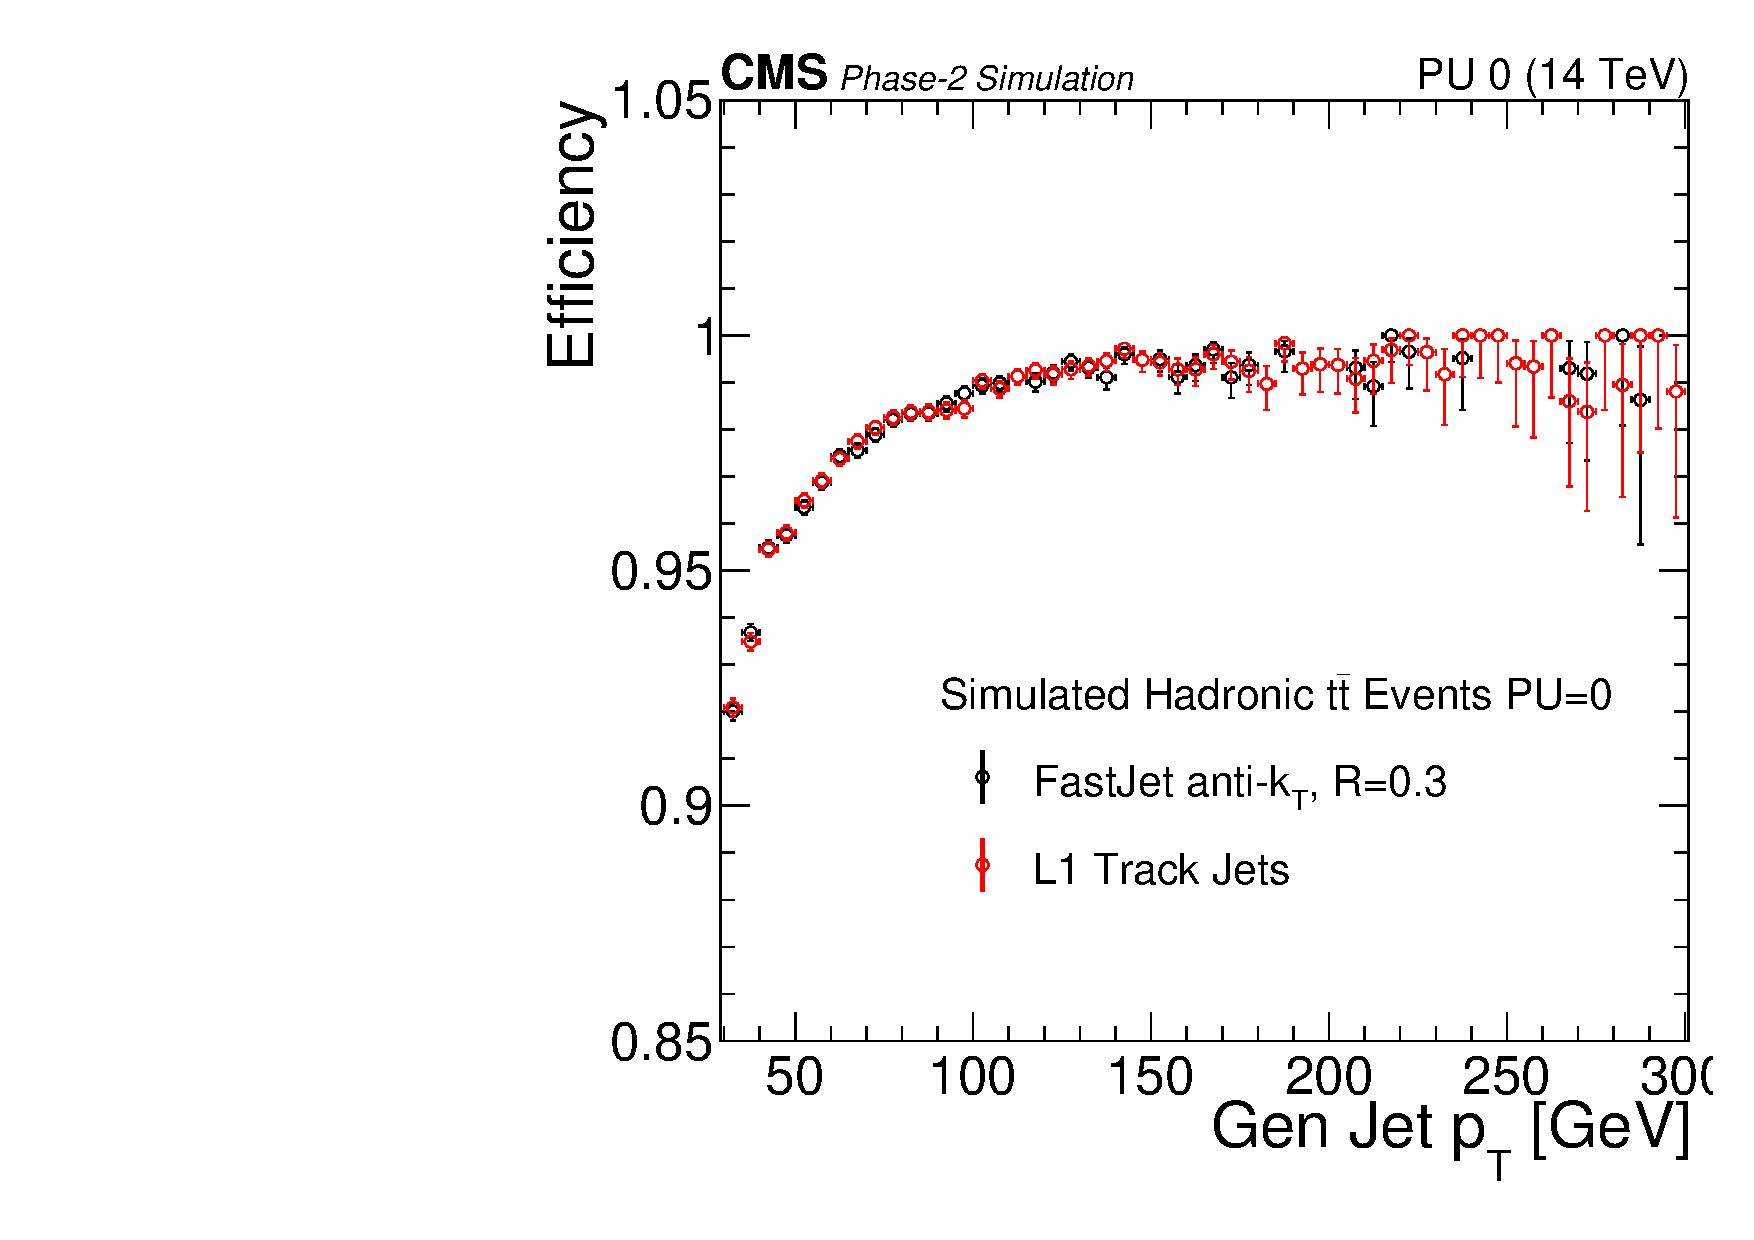
\includegraphics[width=0.45\textwidth]{NoPUTTBarPtEff.pdf}\\
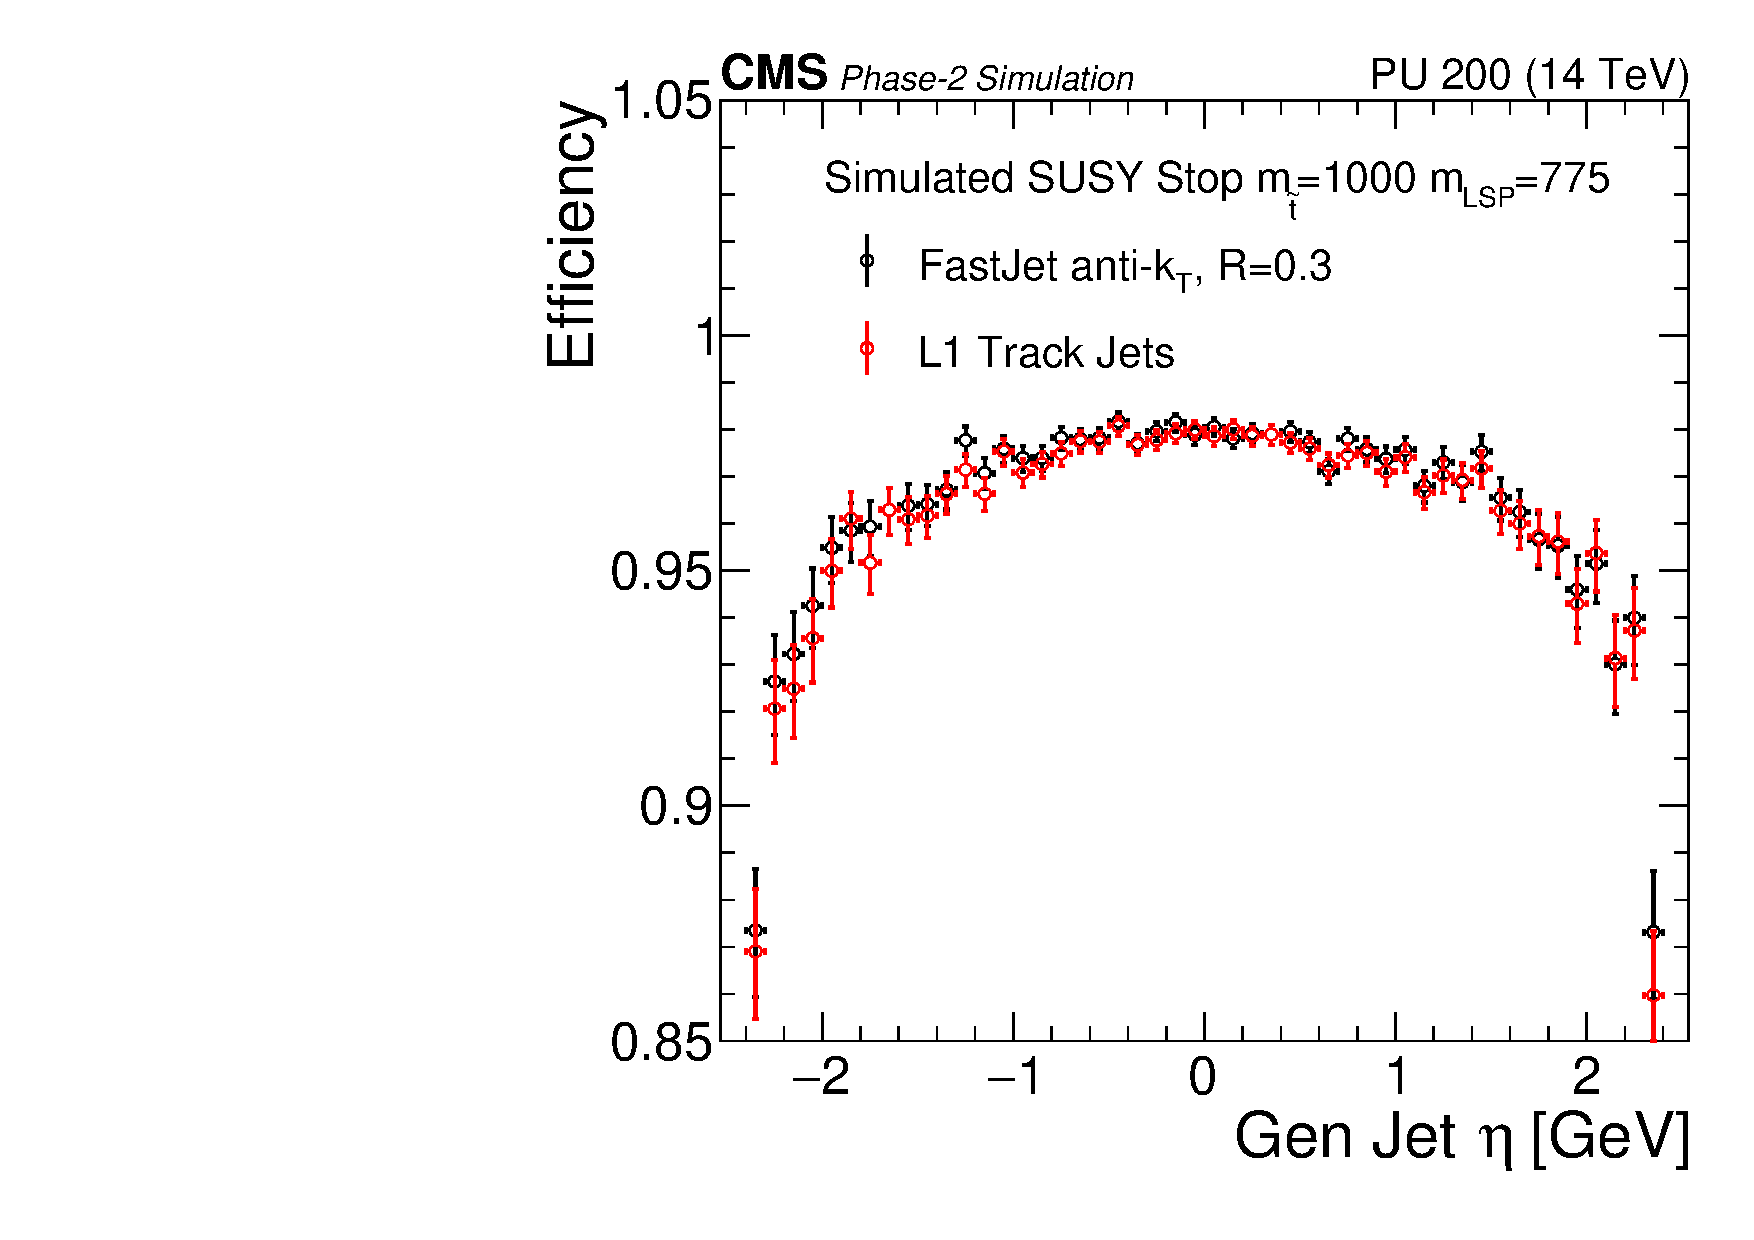
\includegraphics[width=0.45\textwidth]{StopSamplePUEtaEff.pdf}
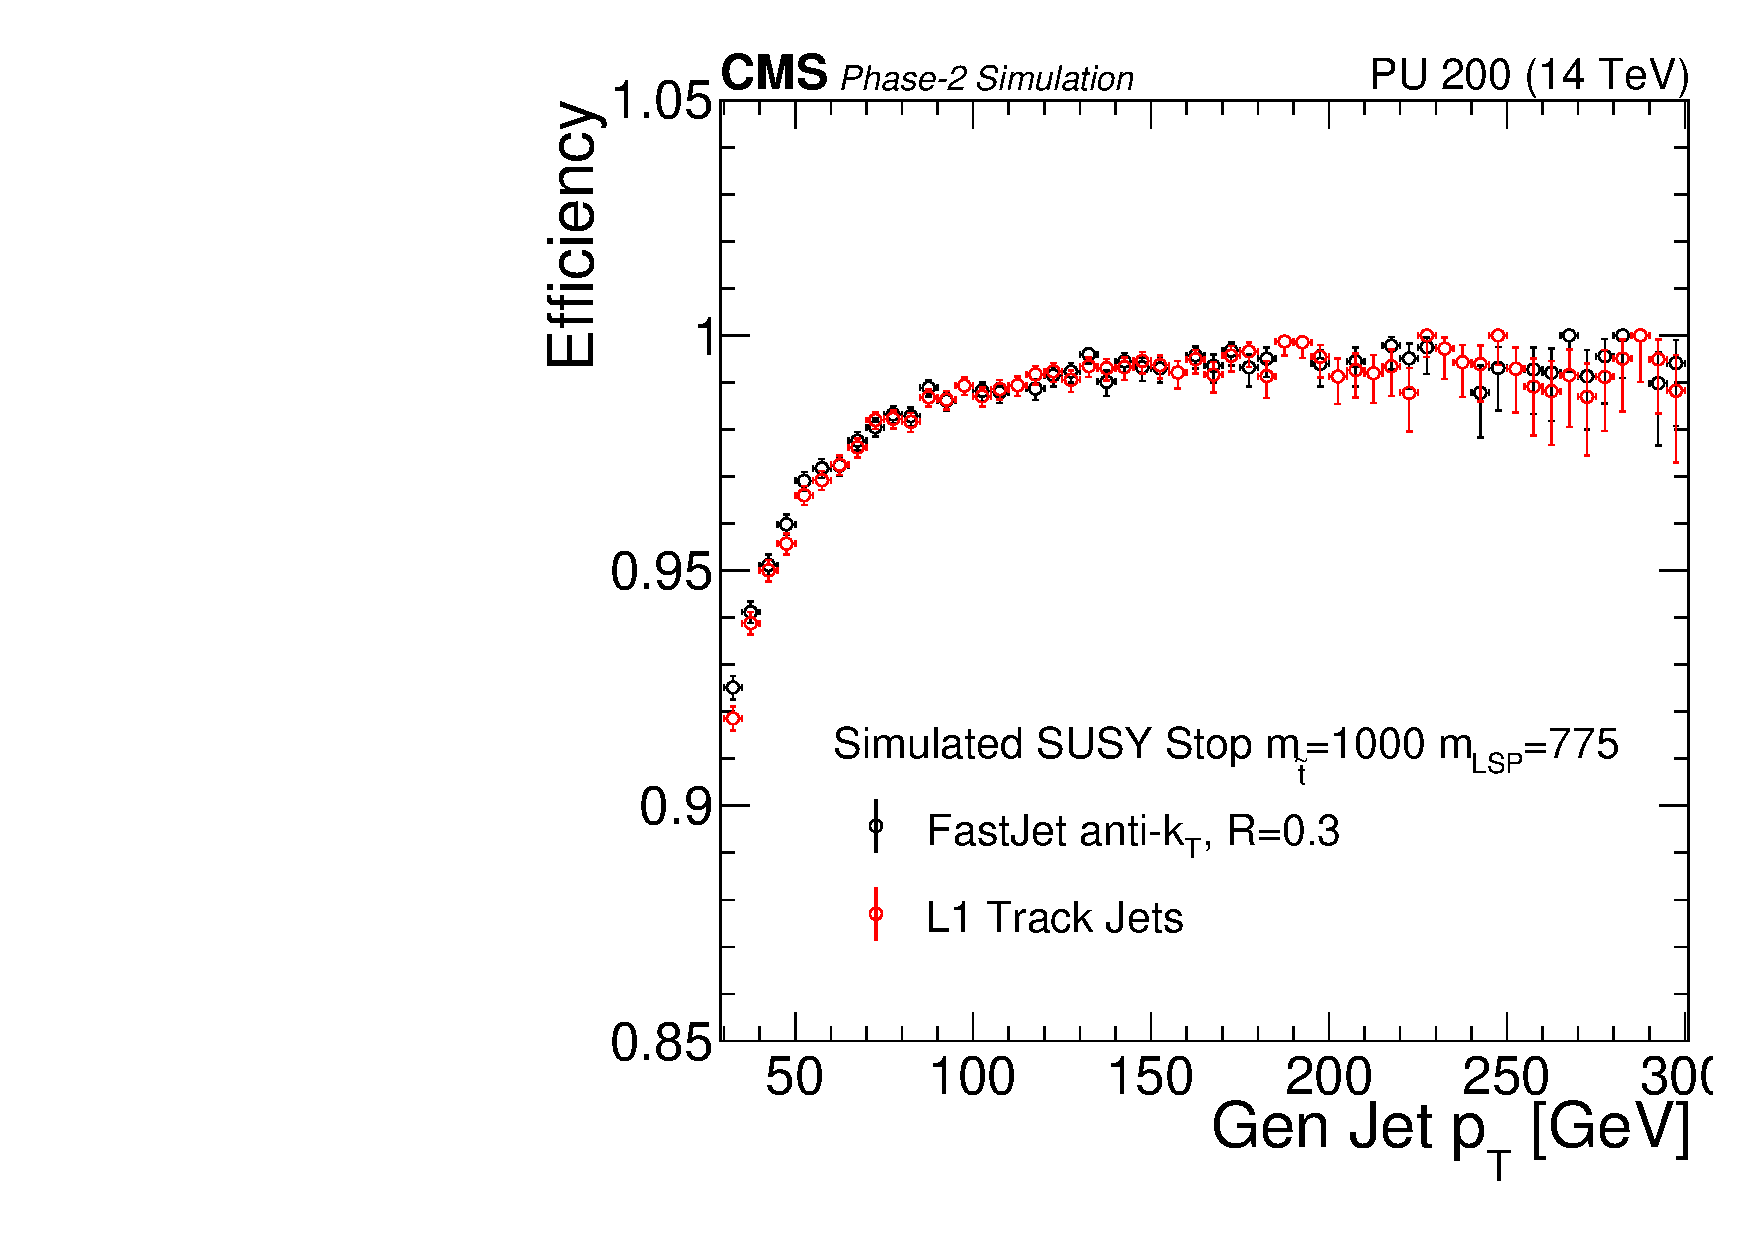
\includegraphics[width=0.45\textwidth]{StopSamplePUPtEff.pdf}
\caption{Comparison of the L1 track jet clustering and anti-$k_{T}$ clustering using FASTJET with $R=0.3$ with the same input collection of L1 reconstructed tracks. (top) The efficiency in fully hadronic t$\overline{t}$ with no pileup events as a function of generator $\eta$(left) and $p_{T}$ (right). The efficiency is computed by matching the generator-level jet to the reconstructed within $\Delta R<0.4$. }
\label{fig:TkJetEfficiency}
\end{figure}


%This section outlines a firmware implemented track clustering algorithm which takes as input a collection of tracks and outputs a collection of track jets. The algorithm does not rely on an input L1 primary vertex position. Instead the clustering is performed in z-regions across the beam spot and flags the jets from the primary collision based on the z-region with the largest track $H_{T}$. 

%The clustering in the $\eta$-$\phi$ plane is done in two 1-Dimensional steps. The first phase of the algorithm parses tracks into 27 $phi$ regions and 24 $\eta$ regions. Tracks are also required to pass the track purity requirements as for the track-based 